\documentclass{article}
\usepackage[spanish]{babel}
\usepackage[numbers,sort&compress]{natbib}
\usepackage{graphicx}
\usepackage{url}
\usepackage{amsmath}
\usepackage{hyperref}
\usepackage{float}
\usepackage{color}
\definecolor{gray86}{gray}{.86}
\definecolor{gray75}{gray}{.75}
\definecolor{gray45}{gray}{.45}
\usepackage{listings}
\lstset{ 
language=C,                
basicstyle=\footnotesize,      
numbers=left,                  
numberstyle=\footnotesize,     
stepnumber=1,                   
numbersep=5pt,                  
backgroundcolor=\color{gray86},  
showspaces=false,              
showstringspaces=false,         
showtabs=false,                
frame=single,           
tabsize=2,          
captionpos=b,          
breaklines=true,        
breakatwhitespace=false,   
escapeinside={\%*}{*)}          
}
\usepackage{subfigure} 
\usepackage[top=15mm, bottom=15mm, left=15mm, right=15mm]{geometry}
\setlength{\parskip}{2mm}
\setlength{\parindent}{0pt}

\author{Abraham Azael Morales Juárez  1422745}
\title{Búsqueda Local}
\date{\today}

\begin{document}

\maketitle

\section{Introducción}
Está práctica se trata sobre fenómenos de coalescencia y fragmentación \cite{REF1}, la coalescencia es la unión de dos elementos conformando uno sólo. Lo que ocasionara que la partícula con el paso del tiempo aumente de tamaño gradualmente \cite{REF2}. Esto es relevante en distintos ámbitos, como, por ejemplo, en el tratamiento de aguas residuales con el uso de filtros.

\section{Objetivos}
Optimizar el código para que se ejecute en el menor tiempo por medio de paralelización.\\
Realizar una gráfica para comparar los tiempos obtenidos de ambos métodos y observar si el ahorro es  significativo para diferentes combinaciones de $k$ y $n$.

\section{Resultados}
Para la realización de esta práctica se tomaron en cuenta distintos parámetros:\\ 
Réplicas de cincuenta.\\
Número de cúmulos $k$ de 5,000, 10,000 y 15,000.\\
Número de partículas $n$ de 500,000, 1,000,000 y 1,500,000.

La paralelización se realizó en la unión de los cúmulos y en la fragmentación de estos. Se coloca sólo un fragmento del código como ejemplo.

\begin{lstlisting}[frame=single]
library(testit) 
library(parallel)
paralelo <- data.frame()
k <- 15000
n <- 1500000
cluster <- makeCluster(detectCores() - 1)

romperse <- function(tam, cuantos) {
  romper <- round(rotura(tam) * cuantos) 
  resultado <- rep(tam, cuantos - romper) 
  if (romper > 0) {
    for (cumulo in 1:romper) { 
      t <- 1
      if (tam > 2) { 
        t <- sample(1:(tam-1), 1)
      }
      resultado <- c(resultado, t, tam - t)
    }
  }
  assert(sum(resultado) == tam * cuantos) 
  return(resultado)
}
\end{lstlisting}
\vspace{40mm}
Los resultados obtenidos son distintos a los esperados, debido a como se observa en la Figura 1, si hay diferencia en los tiempos de ambos métodos pero en la primera iteración, que corresponde a $k$ 5,000 y $n$ 500,000, se observa que el método de paralelización tarda más en comenzar y debido a que son pocos datos los que se están analizando, el método secuencial resulto ser el adecuado.  Por otra parte, en la segunda y tercera iteración, se observa una reducción en los tiempos de la paralelización como se esperaba, esto es debido al aumento en los datos analizados. 

\begin{figure}[H]
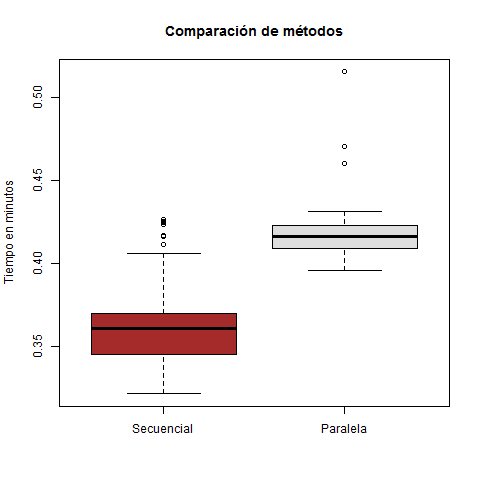
\includegraphics[width=9cm]{500000.png}       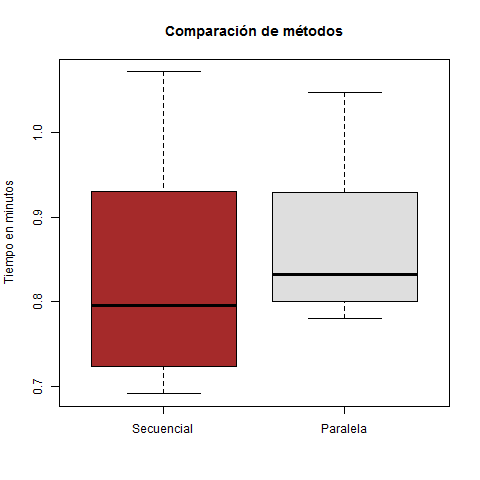
\includegraphics[width=9cm]{1000000.png}
\caption{Comparación de tiempos de las iteraciones $k$ 5,000 y de $n$ 500,000 (lado izquierdo) y de $k$ 10,000 y $n$ de 1,000,000 (lado derecho).}
\end{figure}
\begin{figure}[H]
\centering
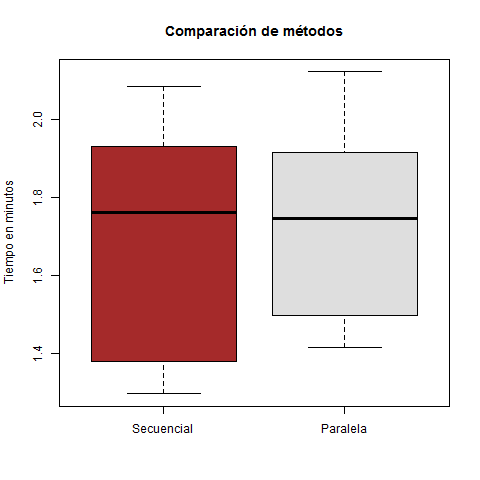
\includegraphics[width=9cm]{1500000.png}      
\caption{Comparación de tiempos de la iteración $k$ 15,000 y de $n$ 1,500,000.}
\end{figure}
\vspace{40mm}
Además se agregan fragmentos del código que corresponde al principio y al final  del análisis.
\begin{lstlisting}[frame=single]
for (replicas in 1:50) {
   inicial1<- Sys.time()
   originales <- rnorm(k)
   cumulos <- originales - min(originales) + 1
   cumulos <- round(n * cumulos / sum(cumulos))
   assert(min(cumulos) > 0)
   diferencia <- n - sum(cumulos)
\end{lstlisting}
\begin{lstlisting}[frame=single]
termino1 <- Sys.time()
    paralelo <- rbind(paralelo, c(termino1-inicial1, k, n, replicas))
  }
names(paralelo) <- c("Tiempo", "Moleculas", "Cumulos", "Replicas")
paralelo$Nivel <- "P"
totaltiempos <- rbind(secuencial, paralelo)
png("Comparacion de metodos.png")
boxplot(totaltiempos$Tiempo~totaltiempos$Nivel, main = "Comparacion de metodos", ylab = "Tiempo en minutos", col = c("brown", "grey87"), names = c("Secuencial", "Paralela"))
graphics.off()
\end{lstlisting}

\section{Conclusiones}
El método de paralelización es efectivo y rápido en comparación del secuencial, sólo si la cantidad de datos es muy grande, lo contrario ocurre cuando los datos son pocos.\\
Se logró la parelelización del código y se demostró la importancia de realizar este método.\\
El método tarda en comenzar debido a que primeramente se dividen las tareas en todos los núcleos para posteriormente realizar el análisis.
Para poder observar mejor los resultados se requiere realizar otros análisis con mayor cantidad de datos.

\bibliographystyle{plainnat}
\bibliography{ref8}




\end{document}